\documentclass[landscape]{sintefposter}

\usepackage{hyperref,multicol,wrapfig}
\usepackage{tcolorbox}

\title{SpliPy$^{1.3}$ - Spline modelling in Python}

\author{Eivind Fonn, Kjetil Andre Johannessen }

\institute{SINTEF Digital, Dept. of Mathematics and Cybernetics, Trondheim, Norway}

\email{Eivind.Fonn@sintef.no, Kjetil.Johannessen@sintef.no}

\conference{SIN\TeX project}

\graphicspath{{.}{Figures/}}

\begin{document}
\leftlogo{splipylogo}
\maketitle

\begin{multicols}{3}
\section{Introduction}
\begin{tcolorbox}[colback=sintefblue!10!white,colframe=sintefblue,title=Abstract]
  Splipy is a pure python library for the creation, evaluation and manipulation of B-spline and NURBS geometries.
  It supports $n$-variate splines of any dimension, but emphasis is made on the use of curves, surfaces and volumes.
  The library is designed primarily for analysis use, and therefore allows fine-grained control over many aspects which is not possible to achieve with conventional CAD tools.
\end{tcolorbox}
\textbf{Keywords:} NURBS, B-splines, CAD, Interpolation, Approximation
\vspace{2cm}

\begin{tcolorbox}[colback=white,colframe=sintefblue,title=Installation]
  The package is distributed through the Python Package Index (PyPI) and can be installed by typing
  \begin{tcolorbox}[colback=sinteflightgrey]
  \begin{verbatim}
> pip install splipy \end{verbatim}
  \end{tcolorbox}
  into the commandline; or anaconda promt
\end{tcolorbox}
The current release is version 1.3

\section{B-splines}
Given a knot vector of nondecreasing knots $\Xi=[\xi_1, \xi_2, \xi_3, ... \xi_{n+p+1}]$ we define the set of $n$ basisis functions by
\begin{tcolorbox}[colback=sintefblue!10!white,colframe=sintefblue,title=The basis]
  \begin{equation}
    \label{eq:bspline}
    N_{i,p}(\xi) = \frac{\xi - \xi_i}{\xi_{i+p}-\xi_i}N_{i,p-1}(\xi) + \frac{\xi_{i+p+1}-\xi}{\xi_{i+p+1}-\xi_{i+1}}N_{i+1,p-1}(\xi),
  \end{equation}
  and,
  \begin{equation}
    \label{eq:bspline-start}
    N_{i,0}(\xi) = \left\{
    \begin{array}{ll}
      1  &  $if $ \ \ \xi \in [\xi_i, \xi_{i+1}) \\
      0  &  $else$
    \end{array}
    \right.
  \end{equation}
\end{tcolorbox}

By creating a tensor product of two or three univariate splines weighted by their controlpoints $\mathbf{B}_{i,j}$, we are able to create surface and solid representations, i.e.
\begin{equation}
  \mathbf{F}(\xi,\eta) = \sum_{i=1}^n \sum_{j=1}^n \mathbf{B}_{i,j} N_{i,p}(\xi)N_{j,q}(\eta)
\end{equation}
for bivariate surfaces.

\begin{center}
  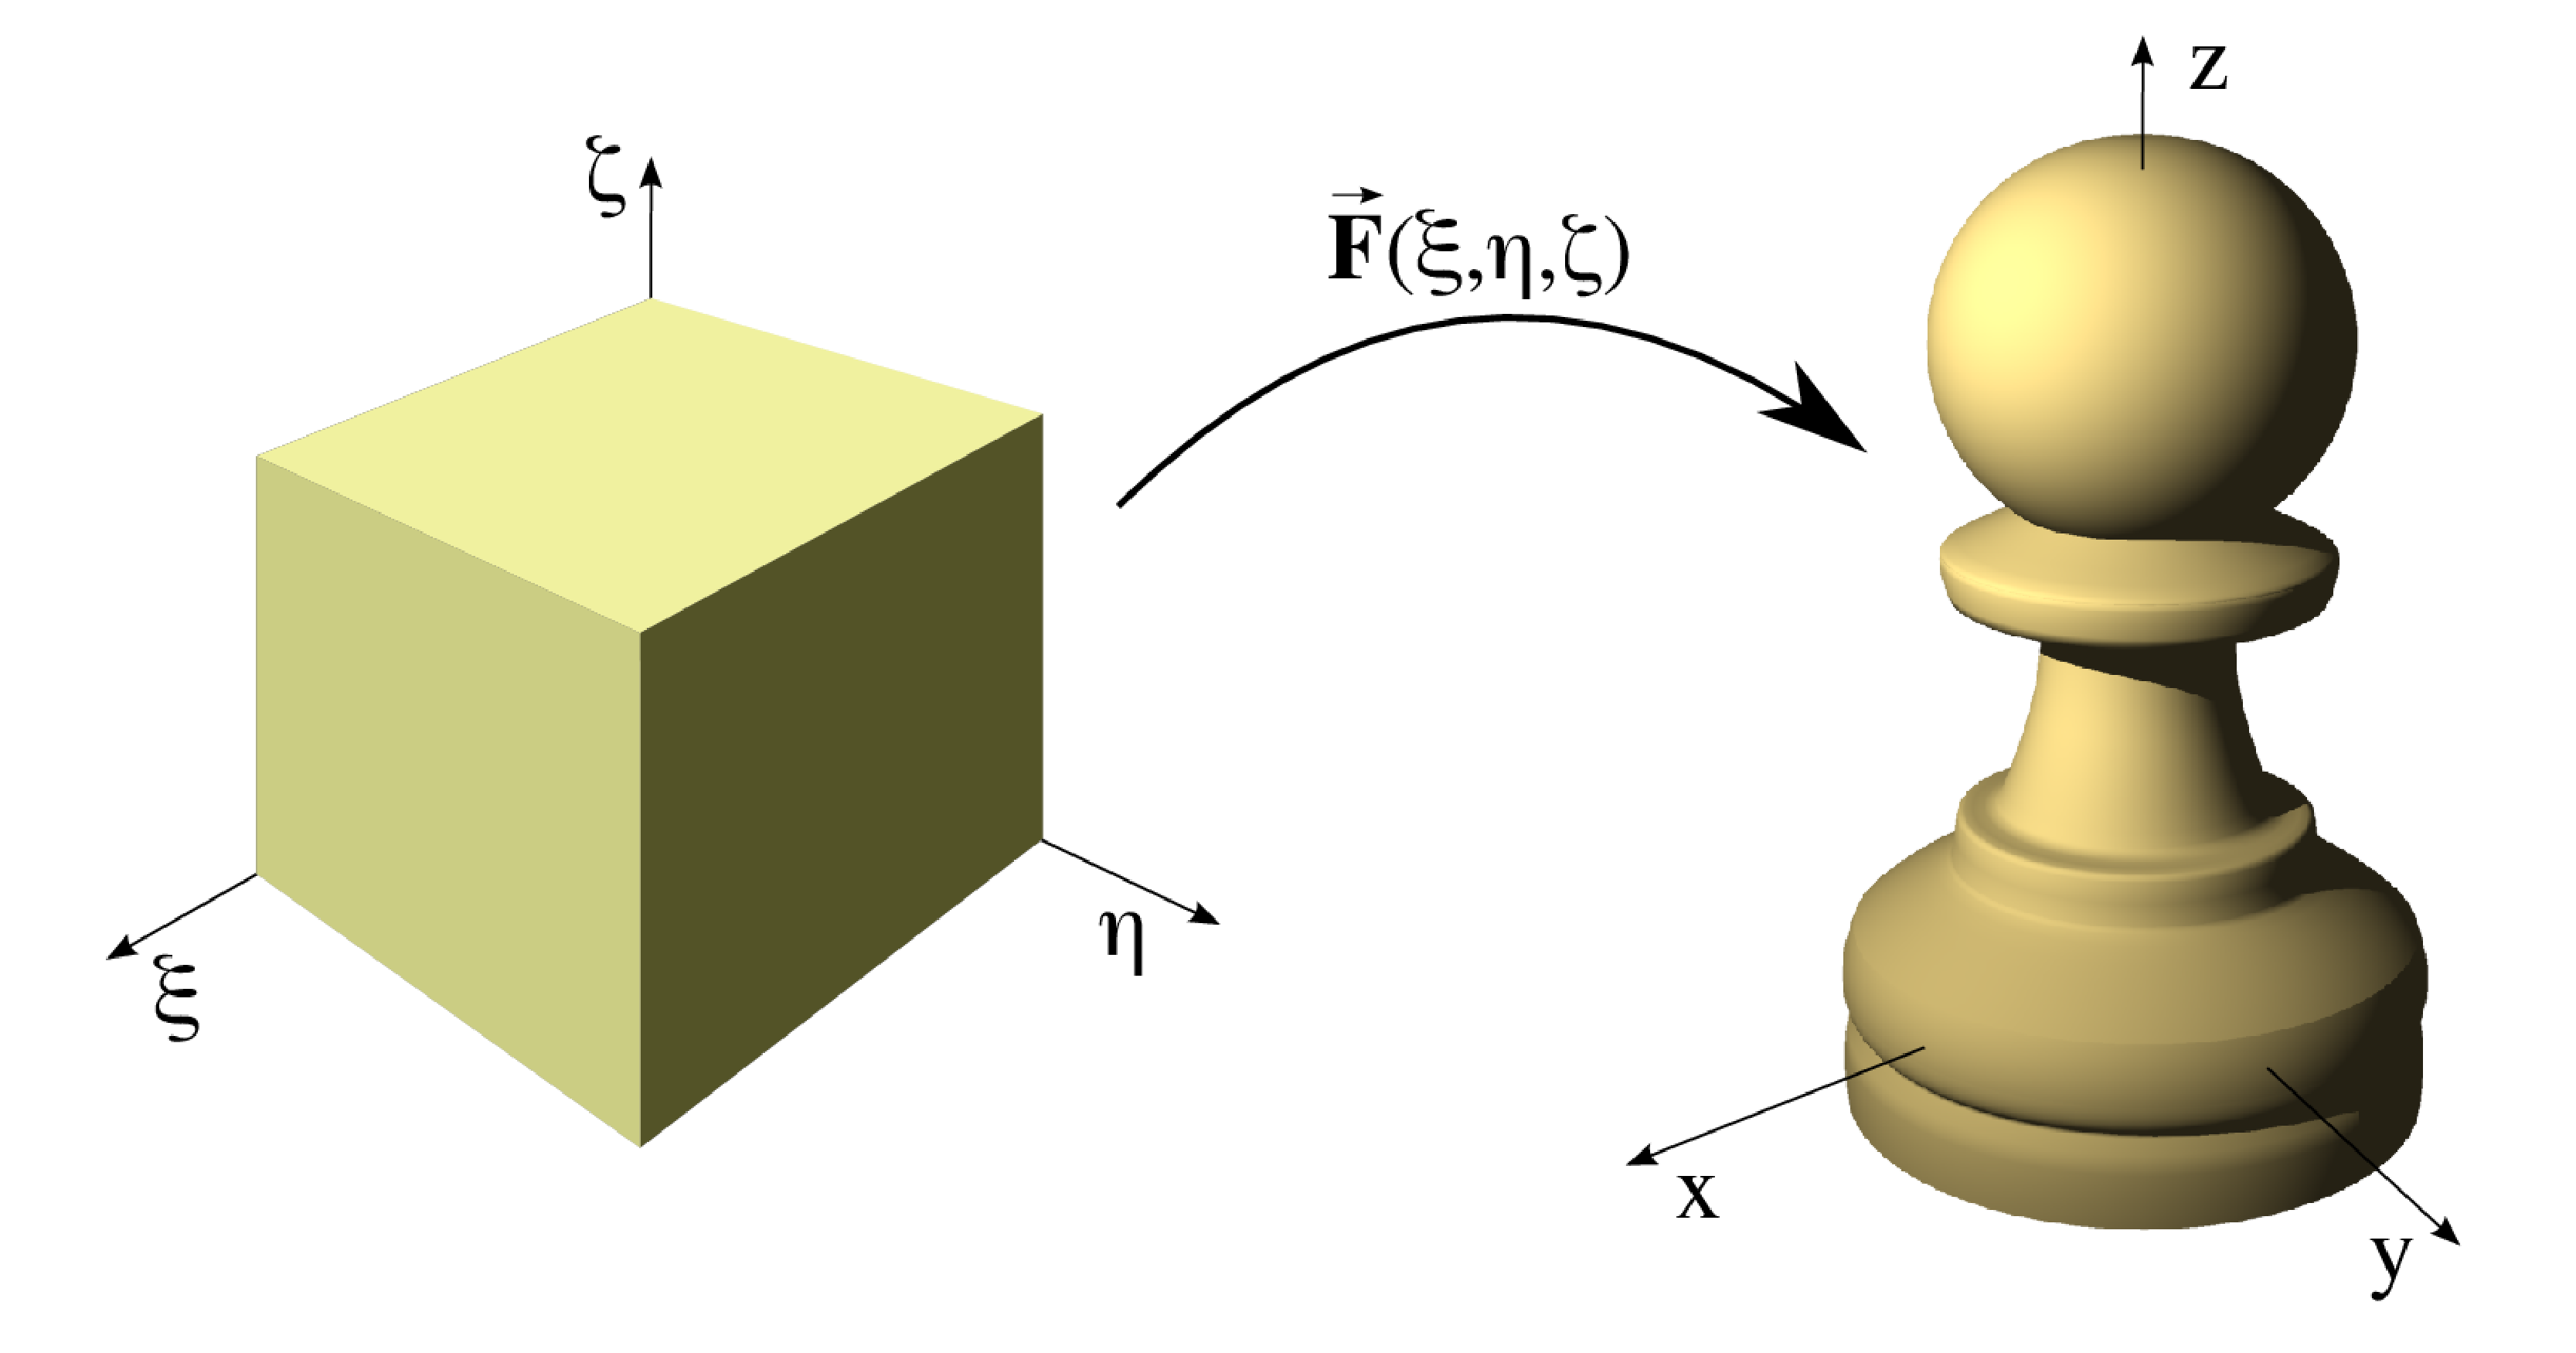
\includegraphics[width=16cm]{pawn-mapping}
  
\includegraphics[height=5cm]{MappingQR} \\
  \normalsize{Fig 1: A trivariate NURBS solid mapping}
\end{center}

\section{Structure}

The class follows a quite simple structure with a Curve, Surface and Volume class which all inherit from a parent SplineObject class. Corresponding to each of these primtitives, we collect a number of generative methods in so-called factory classes.

\begin{center}
  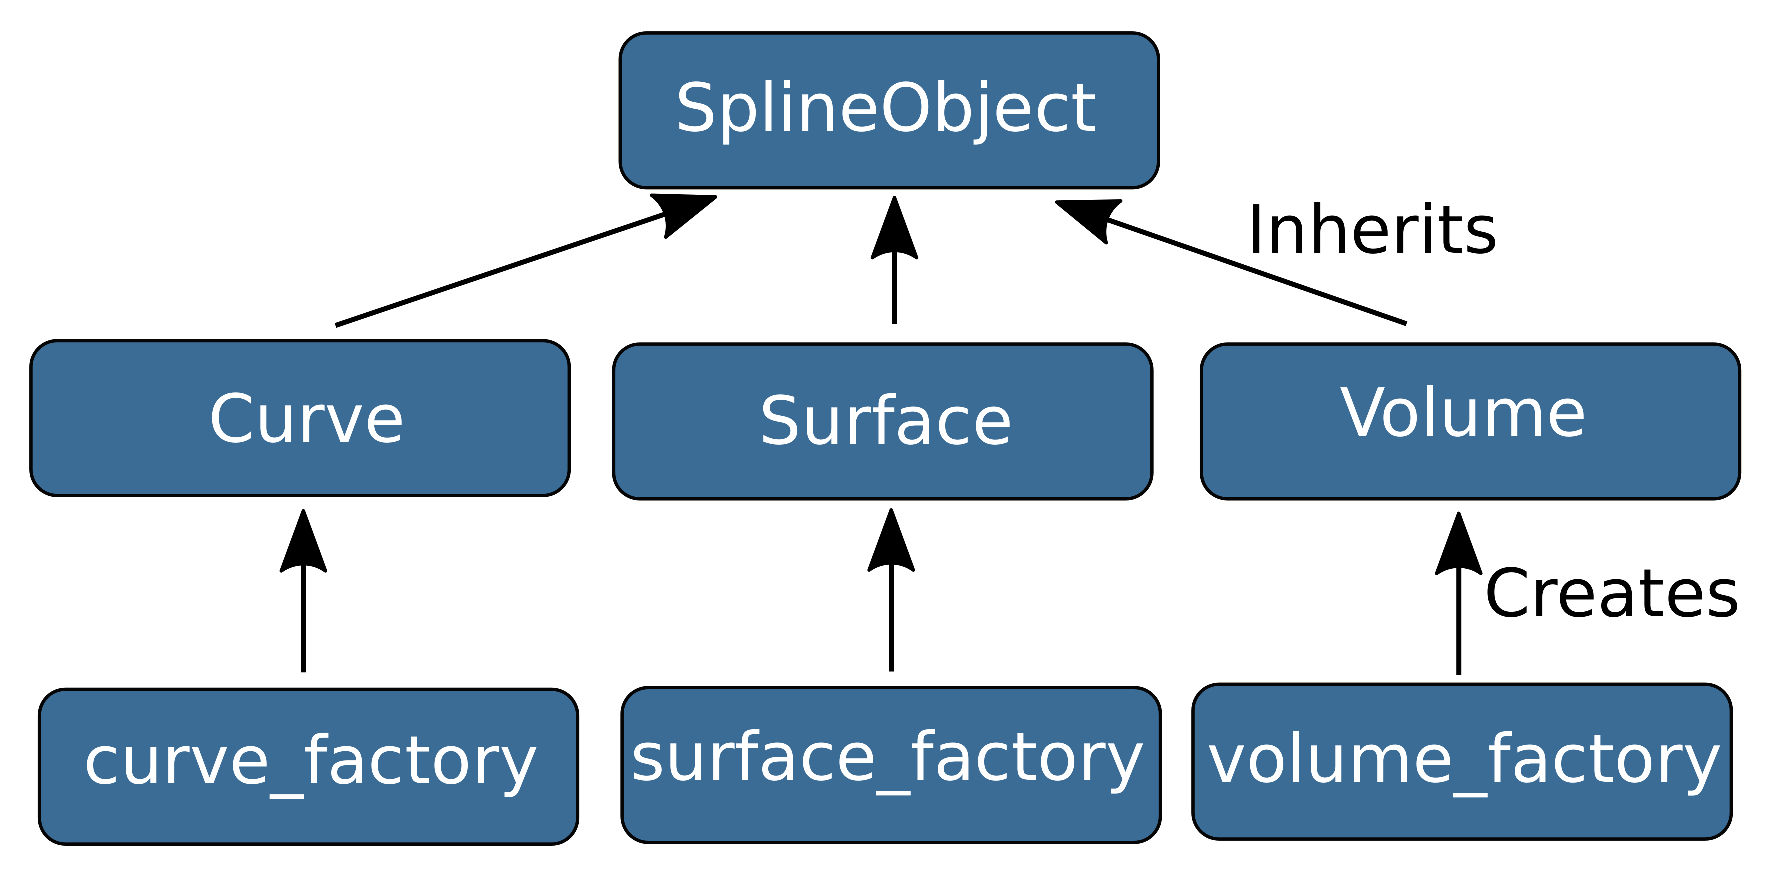
\includegraphics[width=0.7\linewidth]{classstructure} \\
  \normalsize{Fig 2: Primary classes}
\end{center}

\section{Examples}
This allows us to generate mappings from the reference coordinates $(\xi,\eta,\zeta)$ which forms a regular rectangle or box into a complex geometry in physical space given by $(x,y,z)$-coordinates.

\vspace{1cm}

Non-uniform rational B-splines (NURBS) have been a staple technology in \emph{computer aided design} (CAD) for many decades (CITATION NEEDED).
Their mathematical precision allows the user to create smooth parametric descriptions of curves and surfaces, which is necessary in many engineering applications.
Recent years has seen an increased interest in the use of B-splines and NURBS directly in high-fidelity physics simulations such as the finite element method, thereby uniting geometric modelling and analysis.
The groundbreaking work for these methods, termed \emph{isogeometric analysis} (IGA) can be found in \cite{hughes2005iac}.
While commercial CAD tools do well to facilitate NURBS-based modelling, IGA requires finer control of discretization details, and these are often hidden from the user.
We propose Splipy as a modern easy-to-use Python library that will allow scientist and engineers the detailed control that they need to not only make B-spline meshes that are optimized for analysis, but also work well for modelling.

The software allows for rapid generation of high-quality meshes that can be used directly in IGA programs.
While Splipy offers everything needed in terms of basis function evaluations, derivatives etc.~to build a stand-alone finite element solver, we envision that most users will be content to generate the geometry in Splipy followed by exporting to external solvers.

\begin{tcolorbox}[colback=white,colframe=sintefblue,title=Integration with Nutils]
  The package is distributed through the Python Package Index (PyPI) and can be installed by typing
  \begin{tcolorbox}[colback=sinteflightgrey]
  \begin{verbatim}
import splipy.surface_factory as sf
from nutils import *
surf = sf.disc(r=3, center=(2,2))
domain = mesh.rectilinear(surf.knots())
ns = Namespace()
ns.cp = splipy_to_nutils(surf)
ns.phi = domain.basis('spline', p=2)
ns.x = 'phi_n cp_ni'
A = domain.integrate(ns.eval_ij('phi_i,k phi_j,k'))
u = A.solve() \end{verbatim}
  \end{tcolorbox}
  \begin{figure}
    \begin{center}
      
\includegraphics[width=0.4\linewidth]{right.png} \\
      See also: the stand on nutils
    \end{center}
  \end{figure}
\end{tcolorbox}
See more details on the nutils package


\section{Conclusion}

Write som summary things here.
Maybe even box it all in.

{\small \textbf{Disclaimer:}
Splipy does not contain a graphical user interface.
All figures produced on this poster have been created using 3rd party visualizers.
Splipy is to be considered an API ready to be integrated into other custom applications.
}

\end{multicols}

\end{document}

